\documentclass[11pt,letterpaper]{amsart}

\usepackage[utf8]{inputenc}
\usepackage[T1]{fontenc}
\usepackage{lmodern}
\usepackage{amsmath,amssymb,amsthm}
\usepackage{graphicx}
\usepackage{pdfpages}
\usepackage[margin=1.05in]{geometry}
\usepackage[hidelinks]{hyperref}
\usepackage{xcolor}

\hypersetup{
  pdftitle={Monopolar Nodal Operator Framework for the Riemann Hypothesis: Symmetry, Flattening, and Prime-Channel Criteria},
  pdfauthor={German Garcia Andres},
  pdfsubject={Revised nodal-operator edition with monopolar operator, local flattening theorem, and conditional RH closure target}
}

\newtheorem{theorem}{Theorem}
\newtheorem{corollary}{Corollary}
\theoremstyle{definition}
\newtheorem{definition}{Definition}
\newtheorem{remark}{Remark}

\title[Monopolar Nodal Operator Framework]{Monopolar Nodal Operator Framework for the Riemann Hypothesis:\\
Symmetry, Flattening, and Prime-Channel Criteria}
\author{Germ\'an Garc\'ia Andr\'es}
\address{Independent Researcher}
\date{Revised nodal-operator edition - September 2026}

\begin{document}
\maketitle

\begin{abstract}
This revised edition preserves the mathematical body of the Polar Integration manuscript and
adds a final nodal-operator block. The monopolar operator is not introduced here as a new
object: it is the radial \(L=0\) operator architecture already formulated in the original
operator appendix. The new contribution isolates the local nodal mechanism generated by an
amplitude-phase wave
\[
  \psi(\theta)=F(\theta)e^{iG_A(\theta)}
\]
under an involutive angular interpretation \(O_\theta\), phase opposition, and vanishing
transverse quadratic residue \(\operatorname{Tr}_q[X^2]=0\). Under these stated hypotheses the
superposition cancels exactly, \(y+(-y)=0\). This is an exact local cancellation theorem. It is
not, by itself, an unconditional proof of the Riemann hypothesis. The global closure remains
the derivation, without circular insertion of zeros, of a characteristic or perturbation
determinant
\[
  D(z)=E(z)\,\xi\!\left(\frac12+z\right),\qquad E(z)\neq 0,
\]
compatible with the passive-adjoint symmetry used in the operator framework.
\end{abstract}

\section*{Revision Map}

The title has been changed to emphasize the actual architecture of the manuscript:
monopolar operator, nodal flattening, symmetry, and prime-channel criteria. The preserved
source body follows after this page, beginning with its original Section 1. The final pages add
Appendix F and a revised final conclusion. The logical standard remains unchanged: finite
certificates, local cancellation identities, and operator analogies are not promoted to a
global theorem unless the required arithmetic spectral realization is proved independently.

\clearpage

\includepdf[pages=2-33,pagecommand={}]{source_polar_integration_33p.pdf}

\clearpage
\appendix
\section*{Appendix F. General Nodal Theorem for the Monopolar Angular Channel}
\addcontentsline{toc}{section}{Appendix F. General Nodal Theorem for the Monopolar Angular Channel}

\subsection*{F.1. Purpose of the addition}

The preceding manuscript already contains the monopolar operator architecture: the radial
\(L=0\) mode, its collective Hamiltonian, the involution \(J:x\mapsto -x\), and the comparison
with the graph symmetry operator \(P_R\). The present appendix does not introduce a second
operator. It adds the local nodal theorem that explains how an exact cancellation channel is
formed once the angular wave is interpreted through an involutive operator \(O_\theta\).

\begin{definition}[Flattened angular channel]
Let \(\Theta\) be a local parameter space and let
\[
  \psi(\theta)=F(\theta)e^{iG_A(\theta)}
\]
be an amplitude-phase state with real amplitude \(F(\theta)\). Let \(O_\theta:\Theta\to\Theta\)
be an involution,
\[
  O_\theta^2=I.
\]
Let \(y:\Theta\to\mathbb{R}\) denote the local transverse coordinate associated with a chosen
flattening plane \(L\). The channel is called flattened and nodal if
\[
  y(O_\theta\theta)=-y(\theta).
\]
\end{definition}

\begin{definition}[Meaning of \(\operatorname{Tr}_q[X^2]=0\)]
In this appendix the condition
\[
  \operatorname{Tr}_q[X^2]=0
\]
is used as a stated flattening hypothesis: the transverse quadratic residue of the selected
channel vanishes. If \(\operatorname{Tr}_q\) is later specified as a positive Hilbert-space trace
and \(X\) is self-adjoint, this condition is stronger and forces the corresponding quadratic
component to vanish. If \(\operatorname{Tr}_q\) is indefinite, renormalized, or projected, its
domain and positivity properties must be stated before it can be used as a global spectral
criterion.
\end{definition}

\begin{theorem}[General nodal cancellation by angular phase opposition]
Let
\[
  \psi(\theta)=F(\theta)e^{iG_A(\theta)}
\]
be an amplitude-phase state on \(\Theta\). Assume:
\[
  O_\theta^2=I,\qquad y(O_\theta\theta)=-y(\theta),
\]
\[
  F(O_\theta\theta)=F(\theta),
\]
and
\[
  G_A(O_\theta\theta)=G_A(\theta)+\pi \pmod{2\pi}.
\]
If the selected channel also satisfies the flattening condition
\[
  \operatorname{Tr}_q[X^2]=0,
\]
interpreted as vanishing transverse quadratic residue, then the symmetric superposition along
the \(O_\theta\)-pair satisfies
\[
  \psi(\theta)+\psi(O_\theta\theta)=0.
\]
Equivalently, at the level of the real transverse coordinate,
\[
  y(\theta)+y(O_\theta\theta)=y+(-y)=0.
\]
\end{theorem}

\begin{proof}
By amplitude invariance and phase opposition,
\[
\begin{aligned}
  \psi(O_\theta\theta)
  &=F(O_\theta\theta)e^{iG_A(O_\theta\theta)}  \\
  &=F(\theta)e^{i(G_A(\theta)+\pi)}
   =-F(\theta)e^{iG_A(\theta)}
   =-\psi(\theta).
\end{aligned}
\]
Therefore
\[
  \psi(\theta)+\psi(O_\theta\theta)=\psi(\theta)-\psi(\theta)=0.
\]
The coordinate identity follows directly from the imposed involution on the transverse
coordinate:
\[
  y(\theta)+y(O_\theta\theta)=y(\theta)-y(\theta)=0.
\]
The condition \(\operatorname{Tr}_q[X^2]=0\) records that no quadratic transverse residue is
being retained in the flattened channel. Thus the cancellation is exact within the stated local
model.
\end{proof}

\begin{remark}[Local theorem, not automatic global closure]
The theorem proves an exact nodal cancellation once the channel, involution, amplitude
invariance, phase opposition, and residue condition have been fixed. It does not prove that
every nontrivial zero of \(\zeta\) activates this channel. It also does not prove that the
operator determinant is \(\xi\). Those are the global arithmetic and spectral tasks.
\end{remark}

\begin{figure}[p]
\centering
\includegraphics[width=0.97\textwidth]{figures/fig01_aplanamiento_geometrico.png}
\caption{Aplanamiento local. A parabolic or flattened channel is represented by a signed
height \(h_L\) relative to \(L\). The identity \(h_L(R_Lq)=-h_L(q)\) gives exact local
antisymmetry.}
\end{figure}

\begin{figure}[p]
\centering
\includegraphics[width=0.97\textwidth]{figures/fig02_interferencia_nodal.png}
\caption{Interferencia destructiva. Equal amplitudes with phase difference \(\pi\) cancel
exactly: \(h+e^{i\pi}h=0\). This visualizes the nodal channel of the theorem.}
\end{figure}

\clearpage
\section*{Final Revised Conclusion}
\addcontentsline{toc}{section}{Final Revised Conclusion}

The manuscript now contains three logically linked layers. First, the analytic and graph
symmetries isolate the critical fixed set through the involution \(R(s)=1-\overline{s}\) and
the induced graph operator \(P_R\). Second, the monopolar operator architecture supplies an
operator-spectral language based on a radial \(L=0\) mode, an involution, a fixed sector, and
commutation with the corresponding spectral generator. Third, the nodal theorem above supplies
the local cancellation mechanism:
\[
  \psi=F(\theta)e^{iG_A(\theta)},\qquad
  O_\theta^2=I,\qquad
  O_\theta y=-y,\qquad
  \Delta G_A=\pi,\qquad
  \operatorname{Tr}_q[X^2]=0
  \Longrightarrow y+(-y)=0.
\]

Thus the operator is not missing. The new theorem is attached to the existing monopolar
architecture and explains how the flattened channel becomes nodal. What remains as the
decisive closure condition is the arithmetic spectral realization
\[
  D(z)=E(z)\,\xi\!\left(\frac12+z\right),\qquad E(z)\neq 0,
\]
derived from the prime channel and compatible with the passive-adjoint identity
\[
  JAJ^{-1}=-A^*.
\]
If that bridge is proved without assuming RH or inserting the zeros by definition, the
passive-adjoint theorem confines the realized spectral parameters to the imaginary axis and
therefore yields \(\Re\rho=1/2\) for the realized nontrivial zeros. Until that bridge is proved,
the present edition is a coherent nodal-operator framework with exact local cancellations and
explicit global proof obligations.

\[
\boxed{
\text{Monopolar operator}+\text{nodal flattening}+\text{prime-derived determinant}
\Longrightarrow \text{conditional route to RH.}
}
\]

\end{document}
